\documentclass[tikz,border=10pt]{standalone}
\usepackage{fontspec}
\usetikzlibrary{arrows.meta,calc,positioning}

\setmainfont{Latin Modern Roman}

\definecolor{navy}{HTML}{163A5F}
\definecolor{blue}{HTML}{2E6F9E}
\definecolor{amber}{HTML}{A85D00}
\definecolor{slate}{HTML}{536878}
\definecolor{lightblue}{HTML}{F2F7FA}
\definecolor{lightamber}{HTML}{FFF7EC}

\begin{document}
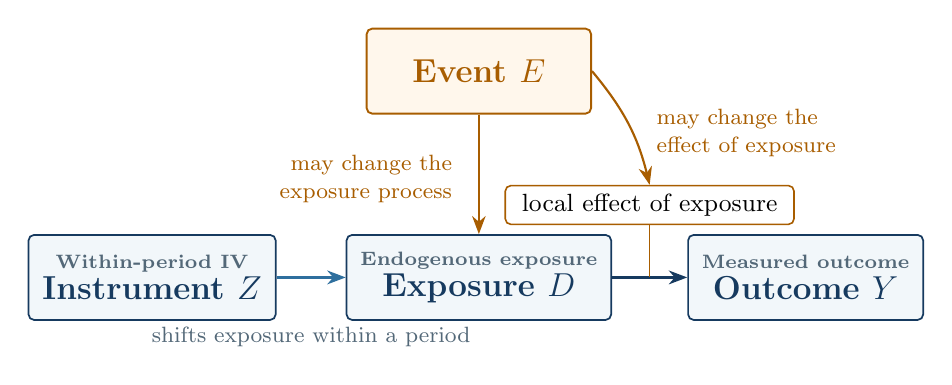
\begin{tikzpicture}[
  x=1cm,
  y=1cm,
  >={Stealth[length=3.2mm,width=2.2mm]},
  lowernode/.style={
    draw=navy,
    fill=lightblue,
    rounded corners=2pt,
    line width=0.62pt,
    minimum width=2.85cm,
    minimum height=1.08cm,
    align=center,
    inner sep=5pt
  },
  eventnode/.style={
    draw=amber,
    fill=lightamber,
    rounded corners=2pt,
    line width=0.68pt,
    minimum width=2.85cm,
    minimum height=1.08cm,
    align=center,
    inner sep=5pt
  },
  effecttag/.style={
    draw=amber,
    fill=white,
    rounded corners=2pt,
    line width=0.58pt,
    align=center,
    inner xsep=6pt,
    inner ysep=3pt,
    font=\fontsize{8.6}{10}\selectfont
  }
]

\node[eventnode] (event) at (0,2.62) {%
  {\fontsize{12}{14}\selectfont\bfseries\color{amber} Event $E$}%
};

\node[lowernode] (instrument) at (-4.15,0) {%
  {\fontsize{7.2}{8.5}\selectfont\bfseries\color{slate} Within-period IV}\\[-1pt]
  {\fontsize{11.6}{13.5}\selectfont\bfseries\color{navy} Instrument $Z$}%
};

\node[lowernode] (exposure) at (0,0) {%
  {\fontsize{7.2}{8.5}\selectfont\bfseries\color{slate} Endogenous exposure}\\[-1pt]
  {\fontsize{11.6}{13.5}\selectfont\bfseries\color{navy} Exposure $D$}%
};

\node[lowernode] (outcome) at (4.15,0) {%
  {\fontsize{7.2}{8.5}\selectfont\bfseries\color{slate} Measured outcome}\\[-1pt]
  {\fontsize{11.6}{13.5}\selectfont\bfseries\color{navy} Outcome $Y$}%
};

\draw[-{Stealth},blue,line width=0.82pt]
  (instrument.east) -- (exposure.west);

\node[font=\fontsize{8.5}{10}\selectfont,color=slate,align=center]
  at ($(instrument.east)!0.50!(exposure.west)+(0,-0.76)$)
  {shifts exposure within a period};

\draw[-{Stealth},navy,line width=0.82pt]
  (exposure.east) -- (outcome.west);

\coordinate (effectpoint) at ($(exposure.east)!0.50!(outcome.west)$);
\node[effecttag] (effect) at ($(effectpoint)+(0,0.92)$)
  {local effect of exposure};
\draw[amber,line width=0.55pt] (effect.south) -- (effectpoint);

\draw[-{Stealth},amber,line width=0.78pt]
  (event.south) --
  node[pos=0.54,left=6pt,font=\fontsize{8.5}{10}\selectfont,color=amber,align=right]
  {may change the\\exposure process}
  (exposure.north);

\draw[-{Stealth},amber,line width=0.78pt]
  (event.east) to[bend left=13]
  node[pos=0.58,right=5pt,font=\fontsize{8.5}{10}\selectfont,color=amber,align=left]
  {may change the\\effect of exposure}
  (effect.north);

\end{tikzpicture}
\end{document}
